\documentclass[border=5pt]{standalone}
\usepackage{fontspec}
\usepackage{unicode-math}
\setmainfont{Noto Serif}
\newfontfamily\FigureItalic{Noto Serif}
\setmathfont{STIXTwoMath-Regular.otf}
\usepackage{tikz}
\usetikzlibrary{arrows.meta,calc,patterns,decorations.pathmorphing,decorations.markings,decorations.pathreplacing,positioning,backgrounds}
\definecolor{Ink}{HTML}{000000}
\definecolor{Curve}{HTML}{000000}
\definecolor{Bzero}{HTML}{000000}
\definecolor{Bone}{HTML}{000000}
\definecolor{Btwo}{HTML}{000000}
\definecolor{Bthree}{HTML}{000000}
\definecolor{Bfour}{HTML}{000000}
\tikzset{
 ax/.style={draw=Ink,line width=.72pt,-{Latex[length=2.4mm,width=1.5mm]}},
 lev/.style={draw=Ink,line width=1.4pt,line cap=butt},
 thinlev/.style={draw=Ink,line width=.65pt,line cap=butt},
 helper/.style={draw=Ink,line width=.65pt},
 bare/.style={draw=Ink,line width=.95pt,dash pattern=on 4pt off 2.8pt},
 curve/.style={draw=Ink,line width=1.85pt,line cap=round,line join=round},
 ray/.style={draw=Ink,line width=1.0pt,-{Latex[length=2.3mm,width=1.4mm]}},
 measure/.style={draw=Ink,line width=.75pt,{Latex[length=1.9mm,width=1.2mm]}-{Latex[length=1.9mm,width=1.2mm]}},
 link/.style={draw=Ink,line width=1.0pt},
 wave/.style={draw=Ink,line width=.85pt,decorate,decoration={snake,amplitude=.33mm,segment length=2.5mm,pre length=.8mm,post length=.8mm}},
 photon/.style={draw=Ink,line width=1.0pt,-{Latex[length=2.0mm,width=1.3mm]},decorate,decoration={snake,amplitude=.4mm,segment length=2.7mm,pre length=0mm,post length=1.9mm}},
 lab/.style={text=Ink,font=\fontsize{13.5}{16}\selectfont,inner sep=2pt},
 small/.style={text=Ink,font=\fontsize{11.5}{14}\selectfont,inner sep=2pt},
 tag/.style={text=Ink,font=\fontsize{14}{17}\selectfont\FigureItalic\itshape,inner sep=2pt}}
\pagestyle{empty}

\begin{document}
% Author schematic: E' is occupied branch, piecewise limiting path.
% CP05: the five E_{i,j} have deliberately different B/W dash patterns,
% while E' is the thick continuous broken line ~0.095 units above the selected branches.
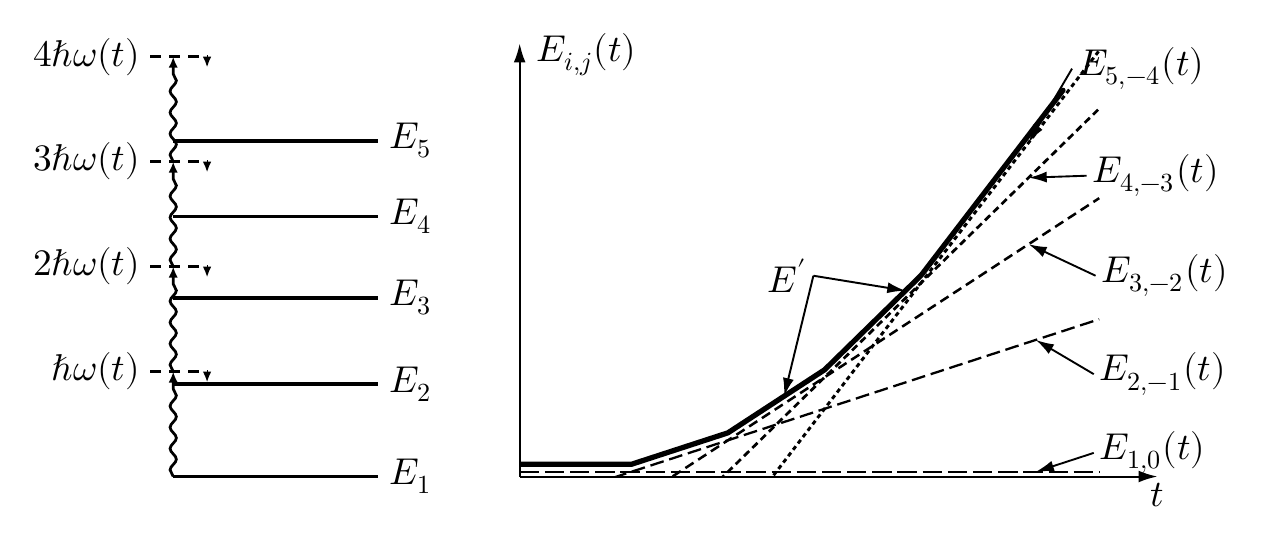
\begin{tikzpicture}[x=1cm,y=1cm]
\coordinate (L0) at (1.65,0.00000);\draw[lev] (L0) -- (4.25,0.00000);\node[lab,anchor=west] at (4.32,0.00000) {$E_{1}$};
\coordinate (L1) at (1.65,1.16960);\draw[lev] (L1) -- (4.25,1.16960);\node[lab,anchor=west] at (4.32,1.16960) {$E_{2}$};
\coordinate (L2) at (1.65,2.27040);\draw[lev] (L2) -- (4.25,2.27040);\node[lab,anchor=west] at (4.32,2.27040) {$E_{3}$};
\coordinate (L3) at (1.65,3.30240);\draw[lev] (L3) -- (4.25,3.30240);\node[lab,anchor=west] at (4.32,3.30240) {$E_{4}$};
\coordinate (L4) at (1.65,4.26560);\draw[lev] (L4) -- (4.25,4.26560);\node[lab,anchor=west] at (4.32,4.26560) {$E_{5}$};
\coordinate (P1) at (1.65,1.33300);\draw[photon,-{Latex[length=1.4mm,width=1.2mm]}] (1.65,0.00000) -- (P1);
\node[lab,anchor=east] at (1.30,1.33300) {$\hbar\omega(t)$};\draw[bare] (1.36,1.33300) -- (2.08,1.33300);\draw[ray,-{Latex[length=1.4mm,width=1.1mm]}] (2.08,1.33300) -- (2.08,1.19300);
\coordinate (P2) at (1.65,2.66600);\draw[photon,-{Latex[length=1.4mm,width=1.2mm]}] (1.65,1.33300) -- (P2);
\node[lab,anchor=east] at (1.30,2.66600) {$2\hbar\omega(t)$};\draw[bare] (1.36,2.66600) -- (2.08,2.66600);\draw[ray,-{Latex[length=1.4mm,width=1.1mm]}] (2.08,2.66600) -- (2.08,2.52600);
\coordinate (P3) at (1.65,3.99900);\draw[photon,-{Latex[length=1.4mm,width=1.2mm]}] (1.65,2.66600) -- (P3);
\node[lab,anchor=east] at (1.30,3.99900) {$3\hbar\omega(t)$};\draw[bare] (1.36,3.99900) -- (2.08,3.99900);\draw[ray,-{Latex[length=1.4mm,width=1.1mm]}] (2.08,3.99900) -- (2.08,3.85900);
\coordinate (P4) at (1.65,5.33200);\draw[photon,-{Latex[length=1.4mm,width=1.2mm]}] (1.65,3.99900) -- (P4);
\node[lab,anchor=east] at (1.30,5.33200) {$4\hbar\omega(t)$};\draw[bare] (1.36,5.33200) -- (2.08,5.33200);\draw[ray,-{Latex[length=1.4mm,width=1.1mm]}] (2.08,5.33200) -- (2.08,5.19200);
\node[tag] at (2.8,-.60) {а};
\draw[ax] (6.05,0) -- (14.15,0) node[lab,anchor=north] {$t$};\draw[ax] (6.05,0) -- (6.05,5.5);\node[lab,anchor=west] at (6.1899999999999995,5.36) {$E_{i,j}(t)$};
\begin{scope}\clip (6.05,.015) rectangle (14.1,5.55);
\draw[bare,draw=Bzero,dash pattern=on 7pt off 2.1pt,line width=0.75pt] plot coordinates {(6.05000,0.06000) (13.41000,0.06000)};
\draw[bare,draw=Bone,dash pattern=on 5pt off 2.1pt,line width=0.83pt] plot coordinates {(6.05000,-0.40250) (13.41000,1.99750)};
\draw[bare,draw=Btwo,dash pattern=on 3.5pt off 2pt,line width=0.91pt] plot coordinates {(6.05000,-1.26500) (13.41000,3.53500)};
\draw[bare,draw=Bthree,dash pattern=on 2.6pt off 1.6pt,line width=0.99pt] plot coordinates {(6.05000,-2.52750) (13.41000,4.67250)};
\draw[bare,draw=Bfour,dash pattern=on 1.6pt off 1.3pt,line width=1.07pt] plot coordinates {(6.05000,-4.19000) (13.41000,5.41000)};
\draw[curve,line width=1.9pt,line join=miter] plot coordinates {(6.05000,0.15500) (7.46833,0.15500) (8.69500,0.55500) (9.92167,1.35500) (11.14833,2.55500) (12.95000,4.90500)};
\end{scope}
\node[lab,text=Bzero,anchor=west] (ql0) at (13.341,0.3) {$E_{1,0}(t)$};\draw[ray,draw=Bzero,line width=.68pt] (ql0.west) -- (12.605,0.06);
\node[lab,text=Bone,anchor=west] (ql1) at (13.341,1.3) {$E_{2,-1}(t)$};\draw[ray,draw=Bone,line width=.68pt] (ql1.west) -- (12.605,1.735000000000001);
\node[lab,text=Btwo,anchor=west] (ql2) at (13.364,2.55) {$E_{3,-2}(t)$};\draw[ray,draw=Btwo,line width=.68pt] (ql2.west) -- (12.512999999999998,2.9499999999999993);
\node[lab,text=Bthree,anchor=west] (ql3) at (13.248999999999999,3.82) {$E_{4,-3}(t)$};\draw[ray,draw=Bthree,line width=.68pt] (ql3.west) -- (12.512999999999998,3.7949999999999973);
\node[lab,text=Bfour,anchor=west] (ql4) at (13.065,5.18) {$E_{5,-4}(t)$};\draw[ray,draw=Bfour,line width=.68pt] (ql4.west) -- (12.512999999999998,4.239999999999997);
\node[lab] (occ) at (9.45,2.55) {$E^\prime$};
\draw[ray,line width=.7pt] (occ.east) -- (9.408,1.0200000000000002);
\draw[ray,line width=.7pt] (occ.east) -- (10.948999999999998,2.3599999999999994);
\node[tag] at (10.05,-.60) {б};
\end{tikzpicture}

\end{document}
